\chapter{Background}
\label{chap:background}

This section gives an overview of related work in literature about feedback exploitation, information-highlighting methods and temporal analysis applications. We also present the system we are extending.

\section{Related Work}

The literature in spatial data analysis has a focus on {\em efficiency} of exploratory interactions. The common approach is to design pre-computed index with enable efficient retrieval of spatial data (e.g., \cite{lins2013nanocubes}). However,
we should also put attention in the {\em value} of spatial data, because is very common to see an analyst getting lost in the huge amount of geographical points. In order to overcome this challenge, visualization environments (e.g., Tableau\footnote{\it http://www.tableau.com}, Exhibit\footnote{\it http://www.simile-widgets.org/exhibit/}, Spotfire\footnote{\it  http://spotfire.tibco.com}) offer features to manipulate data (e.g., filters, aggregate queries, etc).

\subsection{Feedback exploitation}

Our proposed spatial-temporal model leverage the spatial data analysis by exploiting collected feedback during the analyst exploration to highlight subsets of geographical points. In the literature, are several instances of feedback exploitation to guide the analysts in further analysis steps (e.g., \citeonline{boley2013one}). \todo{REWRITE THE FOLLOWING} The common approach is a top-$k$ processing methodology in order to prune the search space based on the explicit feedback and recommend a small subset of interesting results of size~$k$. A clear distinction of our work is that it doesn't aim for pruning, but leveraging the actual data with potential interesting results that the analyst may miss due to the huge volume of spatial data. While in top-$k$ processing algorithms, analyst choices are limited to $k$, we offer the freedom of choice where highlights get seamlessly updated with new analyst choices.

\subsection{Information-highlighting methods}

\todo{TALK ABOUT EACH ONE}
There exist few instances of information-highlighting methods in the literature: \citeonline{Liang2010,Robinson2011,wongsuphasawat2016voyager,willett2007scented}. All these methods are {\em objective} and do not apply to the context of spatial guidance where user feedback is involved. In terms of recommendation, few approaches focus on spatial dimension \cite{Bao2015,Levandoski:2012} while the context and result diversification are missing.

\subsection{Temporal analysis applications}

\todo{TALK ABOUT EACH ONE}
There are currently several instances which combine temporal analysis with spatial data in the literature (e.g., \citeonline{baculo2017,balahadia2017,chidean2018,ghahramani2018,kamath2013,lopestexeira2018,ma2017,mijovic2016,tomoki2010,nara2007,zhan2017,zheng2018}). Those are applications of temporal analysis in specific context, which does not involve user feedback, but represent how temporal analysis could be insightful.

\citeonline{baculo2017} and \citeonline{balahadia2017} make use of public data of Manila, the most densely populated city in the Philippines, to combine spatial data, temporal analysis and prediction model to allow decision makers to prepare an effective public management plan. \citeonline{ma2017} and \citeonline{zheng2018} also perform real-world analyses of how events (e.g., protests) impact the taxi trajectories which results could provide helpful insights for traffic control and transit service plans for city administrators. Both perform insightful analyses which we will use as inspiration.

\citeonline{chidean2018} present how to detect spatial-temporal patterns in the context of wind power resource in the Iberian Peninsula using Second-Order Data-Coupled Clustering algorithm. Despite the detailed study, it does not work in a exploratory context.

\citeonline{ghahramani2018}, \citeonline{lopestexeira2018} and \citeonline{zhan2017} demostrate how temporal analyses can be applied in the geographical context. \citeonline{zhan2017} goes deeper generating a hierarchical cluster tree. Regardless of insights and methods, it does not contribute to the subject in question.

\citeonline{kamath2013} propose a novel reinforcement learning approach to predict events (i.e., online meme) in the spatial-temporal context.

\citeonline{nara2007} introduce a 3D visualization of space-time which helps to qualitatively and quantitatively analyze the spatiotemporal patterns and tendencies. We will make use of this visualization approach to display our collected data in chapter \ref{chap:collecting}.

\section{GeoGuide}

\begin{figure}[t]
	\centering
	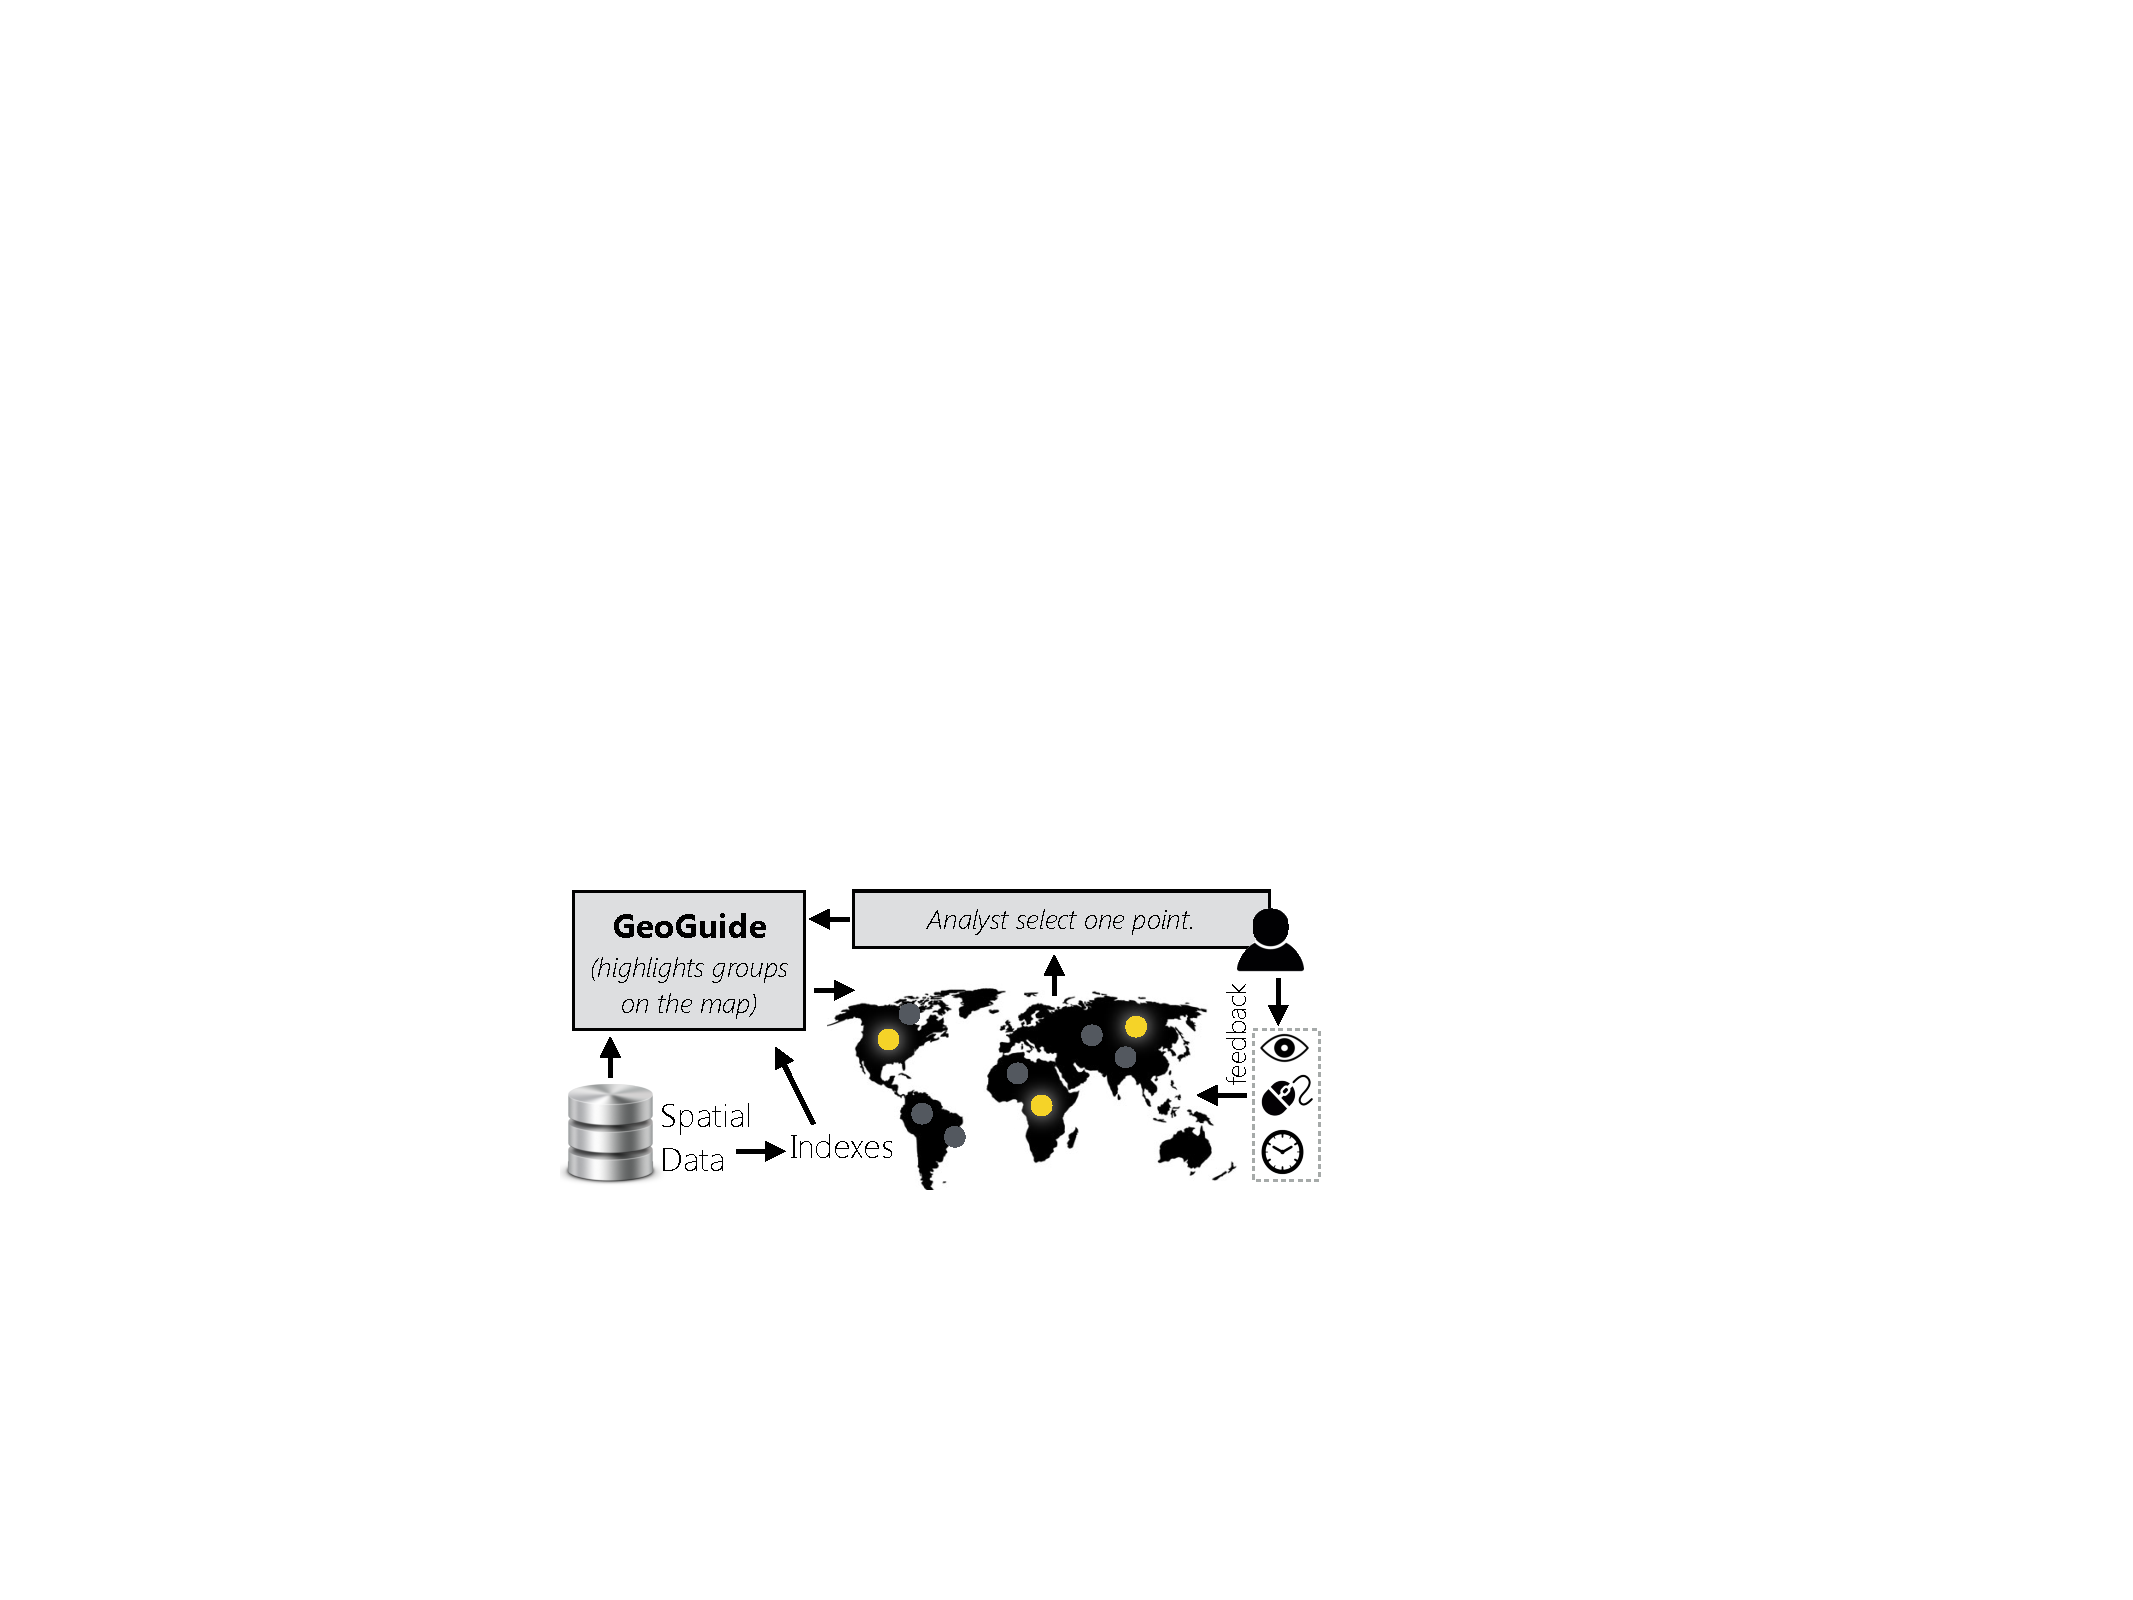
\includegraphics[width=\columnwidth]{imagens/framework}
	\caption{GeoGuide Framework}
	\label{fig:framework}
	\vspace{-10pt}
\end{figure}

GeoGuide \cite{omidvarTehrani2017} is a spatial data visualization environment which keep track of user preferences during exploration in order to use collected feedback to highlight subsets of geographical points that may be interesting to the analyst. Figure \ref{fig:framework} illustrates the main components of GeoGuide architecture which we will present in the next subsections.

\subsection{Preprocessing}

GeoGuide requires a preprocessing step in order to create a index which will be used during highlighting. The index is a comparative table between every points with two quality metrics, i.e., relevance and diversity.

\subsubsection{Relevance}

Relevance represent how a point $a$ is similar to a point $b$ in the current dataset. GeoGuide use the relevance to highlight points in the same line with the analyst feedback.

\subsubsection{Diversity}

Diversity represent how distant is the region where a point $a$ is to the region where point $b$ is located. It allow the analyst to explore different regions, but still work with relevant points to his interest.

\subsection{Tracking User Preferences}

In order to keep track of user preferences, GeoGuide use both explicit and implicit feedback. Explicit feedback is when the user is analyzing the attributes of a point (e.g., the house description in a Airbnb context) and explicitly ask to explore similar points to the current selected one. Implicit feedback is tracked using the mouse movements, gaze tracking and metrics like ``how long the user was analysing the profile of a point''.

\subsection{Highlighting Spatial Data}

GeoGuide combine both preprocessed index and user preferences to highlight a subset of spatial data according to the analyst preferences. GeoGuide highlighting feature prove to be efficient in terms of ``how many steps the analyst takes until complete a task of finding a point in a request location''. Using GeoGuide the analysts were able to complete the task using in average 10.7 steps, while using Tableau, they took about 43 steps.

\vspace{25pt}

\noindent In this work, we will leverage GeoGuide into two new concepts: $i$. interesting dense regions and $ii$. understanding how the user preferences change over time.

